%%%%%%%%%%%%%%%%%%%%%%%%%%%%%%%%%%%%%%%%%%%%%%%%%%%%%%
%\section{Human Activity Recognition}
%%%%%%%%%%%%%%%%%%%%%%%%%%%%%%%%%%%%%%%%%%%%%%%%%%%%%%

\subsection{Method}

\subsection{Related Work}
Explain common approaches to human activity recognition, evaluation
methods and resulted quality.

\subsection{Component Description}
Explain our own implementation:

\begin{enumerate}
\item Architecture Description (Class diagrams, DB Schemes)
\item Decision Tree classifier
\item PCA-SVM based classifier
\end{enumerate}

\begin{figure}[htbp]
\centering
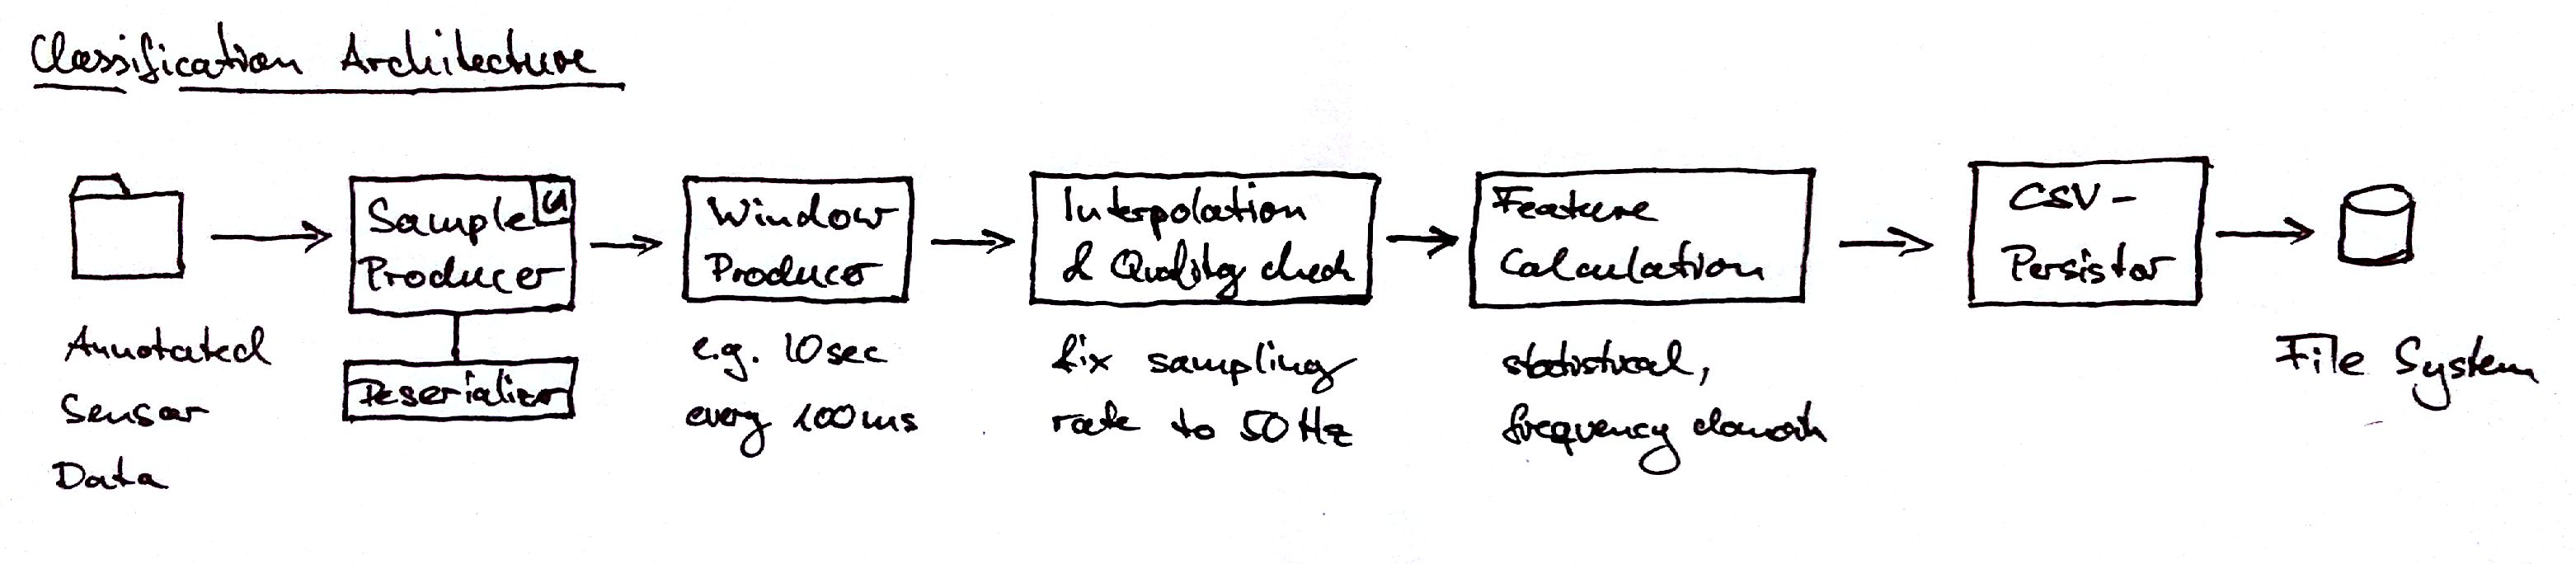
\includegraphics[width=\textwidth]{img/har/classification_architecture.jpg}
\caption{Classification Architecture}\label{fig:classification_architecture}
\end{figure}

\begin{figure}[htbp]
\centering
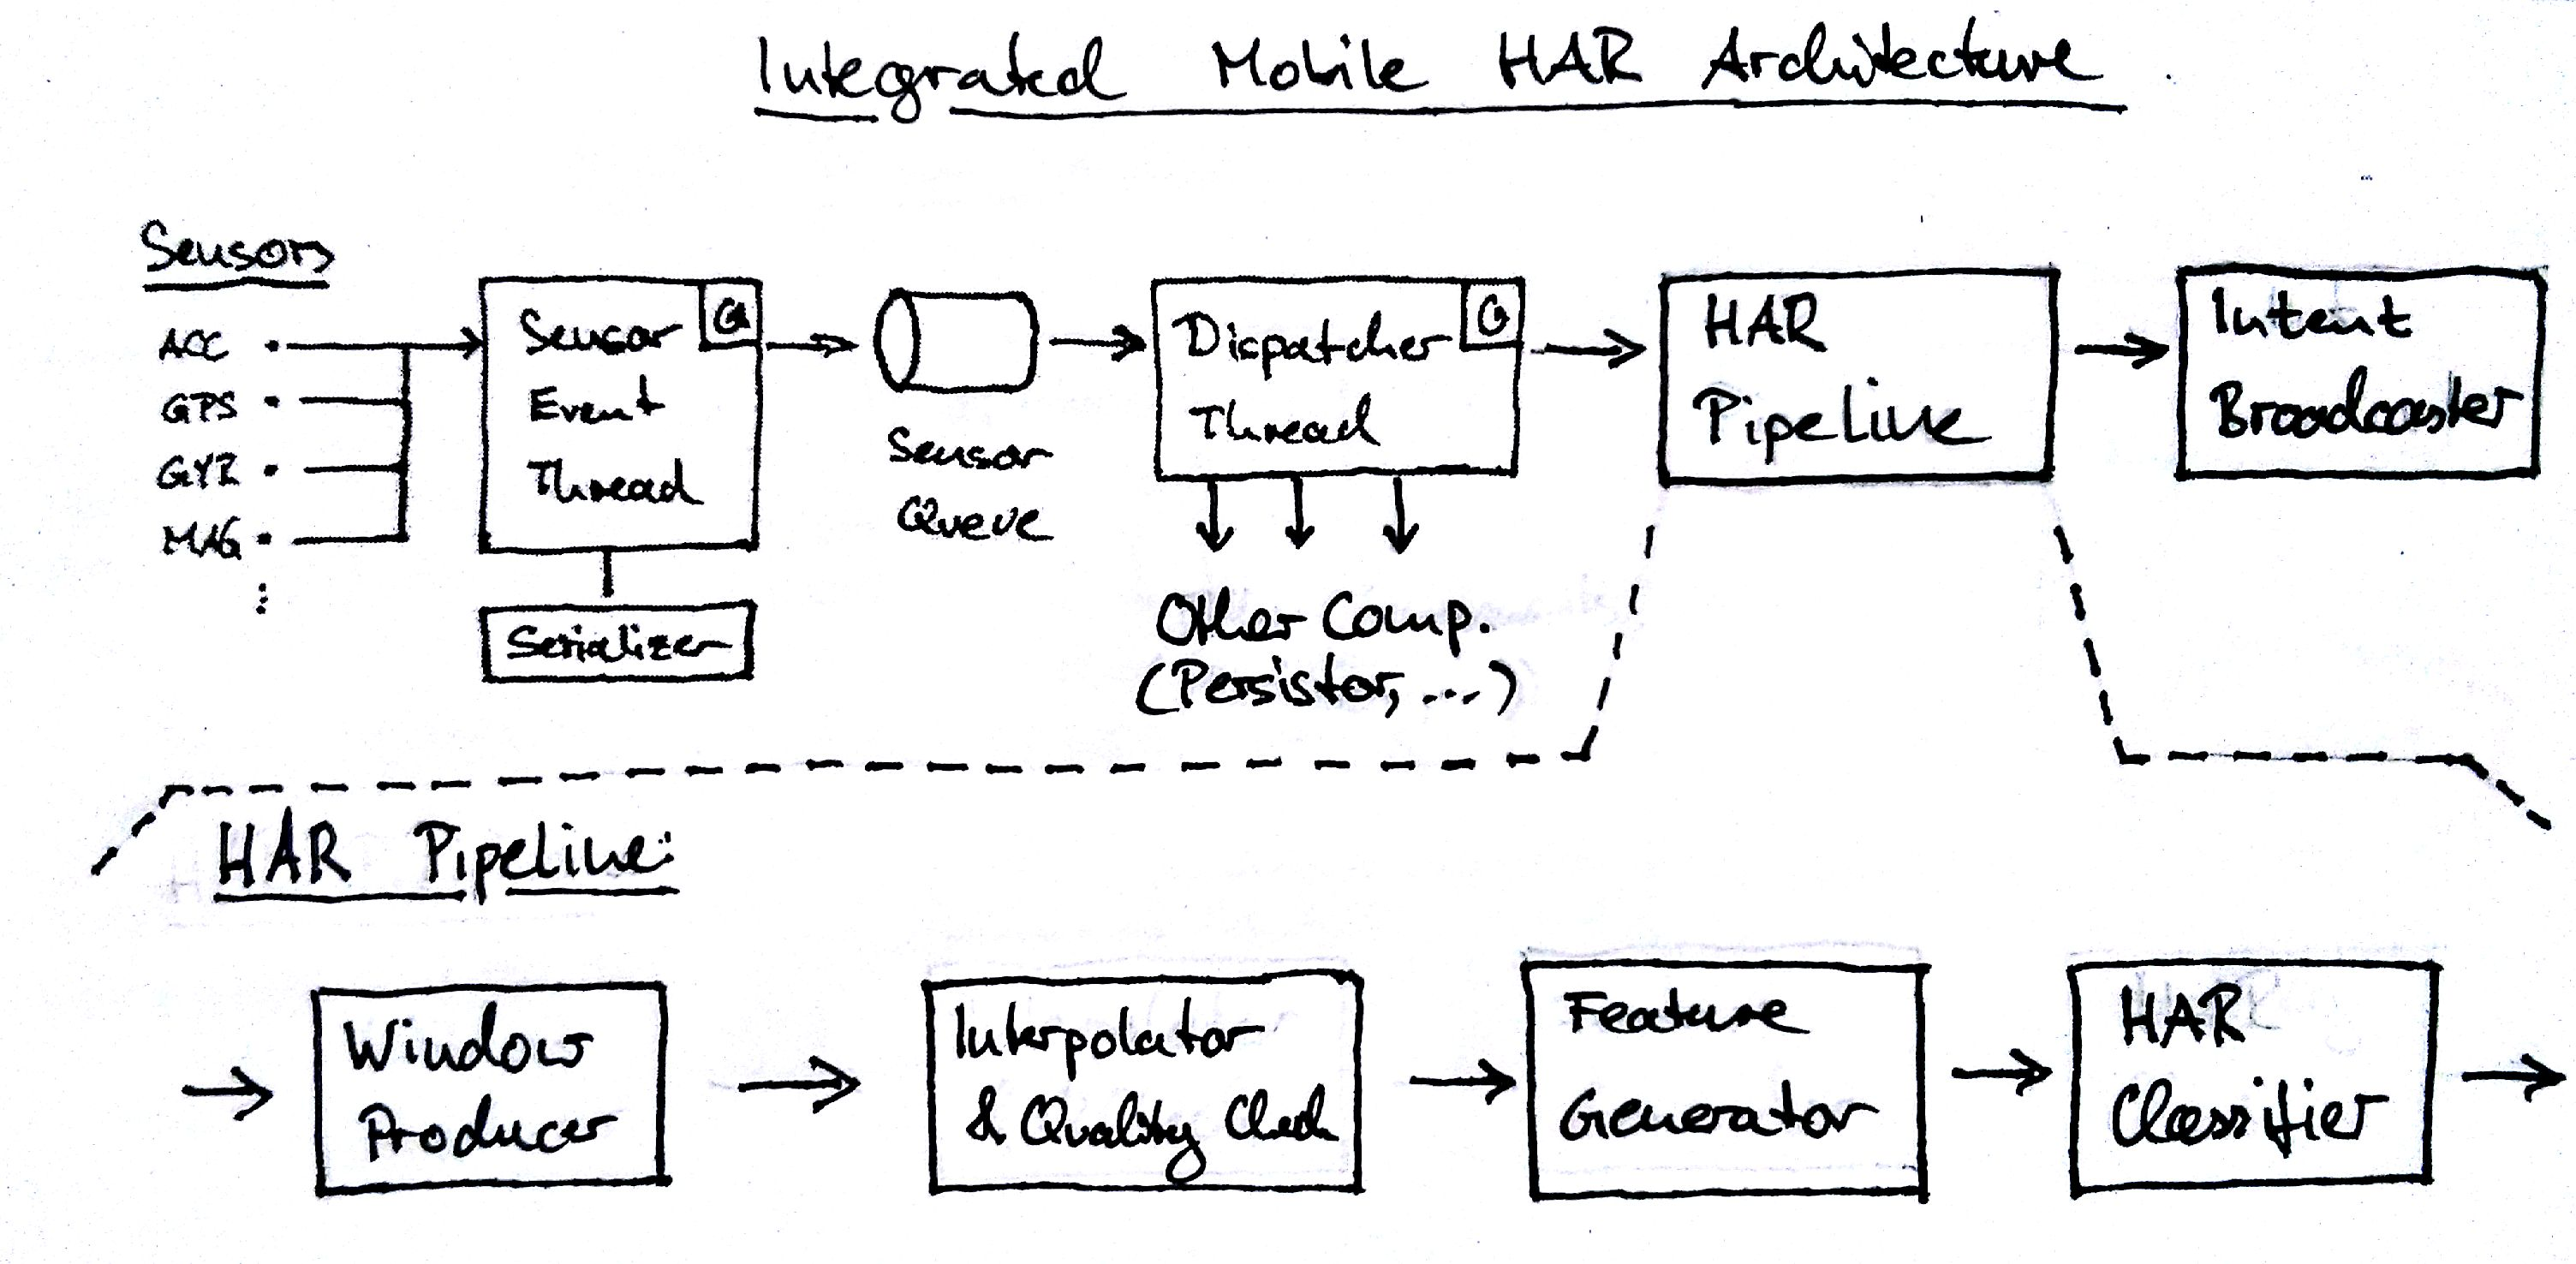
\includegraphics[width=\textwidth]{img/har/integration.jpg}
\caption{Integrated HAR Architecture}\label{fig:integrated_har}
\end{figure}


\subsection{Cross-Platform Strategy}
Explain problems with Titanium framework.

Android component runs on Blackberry. 

Implement HAR as SAAS. Write client app for iOS.

\subsection{Evaluation}
Comparison of our classifier with literature on the basis of external
data sets.


%%% Local Variables:
%%% mode: latex
%%% TeX-master: "../D1-2"
%%% End:
